%%%%%%%%%%%%%%%%%%%%%%%%%%%%%%%%%%%%%%%%%
% baposter Landscape Poster
% LaTeX Template
% Version 1.0 (11/06/13)
%
% baposter Class Created by:
% Brian Amberg (baposter@brian-amberg.de)
%
% This template has been downloaded from:
% http://www.LaTeXTemplates.com
%
% License:
% CC BY-NC-SA 3.0 (http://creativecommons.org/licenses/by-nc-sa/3.0/)
%
%%%%%%%%%%%%%%%%%%%%%%%%%%%%%%%%%%%%%%%%%

%----------------------------------------------------------------------------------------
%	PACKAGES AND OTHER DOCUMENT CONFIGURATIONS
%----------------------------------------------------------------------------------------

\documentclass[portrait,a0paper,fontscale=0.35]{baposter} % Adjust the font scale/size here : fontscale=0.285
\usepackage{textpos}
\usepackage[frenchb]{babel}
\usepackage[T1]{fontenc}
\usepackage[utf8]{inputenc}
\usepackage{tikz}
\usepackage{graphicx} % Required for including images
%\graphicspath{{Figures/}} % Directory in which figures are stored
\usepackage{amsmath} % For typesetting math
\usepackage{amsthm}
\usepackage{amssymb} % Adds new symbols to be used in math mode
\usepackage{booktabs} % Top and bottom rules for tables
\usepackage{enumitem} % Used to reduce itemize/enumerate spacing
\usepackage{palatino} % Use the Palatino font
\usepackage[font=small,labelfont=bf]{caption} % Required for specifying captions to tables and figures
\usepackage{multicol} % Required for multiple columns
\usepackage{tikz} % Required for flow chart
\usetikzlibrary{shapes,arrows} % Tikz libraries required for the flow chart in the template
\usepackage{dsfont}
\usepackage{listings}
\usepackage{subfigure}
\usepackage{color}
\usepackage{nth}
\usepackage{a4wide}
\usepackage{graphicx,color}
\usepackage{array}
\usepackage[nottoc, notlof, notlot]{tocbibind}
\usepackage{subfigure}
\usetikzlibrary{arrows,shapes,positioning,calc}
%\definecolor{CPU}{RGB}{30, 167, 223}
%\definecolor{CPU}{RGB}{8, 138, 104}
\definecolor{gris}{gray}{0.9}
\usepackage{geometry}
\geometry{left=0.5cm,right=0.5cm,bottom=0.5cm,top=0.5cm,centering}
\usepackage{subfig}
\usepackage{float}
\usepackage{multicol}
\usepackage{enumitem,rotating}
\usepackage{bbm}
\usepackage{wrapfig}


\newcommand{\sidecap}[1]{ {\begin{sideways}\parbox{0.2\textwidth}{\centering #1}\end{sideways}} }

\theoremstyle{plain}
\newtheorem*{thm}{Theorem}
%\theoremstyle{definition}
%\newtheorem*{defi}[thm]{Definition}
\theoremstyle{plain}
\newtheorem*{prop}{Properties}
\theoremstyle{plain}
\newtheorem*{hyp}{Assumption}
\theoremstyle{plain}
\newtheorem*{proposition}{Proposition}

\setlength{\columnsep}{1.5em} % Slightly increase the space between columns
\setlength{\columnseprule}{0mm} % No horizontal rule between columns

\definecolor{lightred}{rgb}{0.5 0 0}

\newcommand{\compresslist}{ % Define a command to reduce spacing within itemize/enumerate environments, this is used right after \begin{itemize} or \begin{enumerate}
\setlength{\itemsep}{1pt}
\setlength{\parskip}{0pt}
\setlength{\parsep}{0pt}
}

\definecolor{CPU}{RGB}{0, 153, 125} % Defines the color used for content box headers




% Math operators
\newcommand{\scal}[2]{\left\langle #1 , #2 \right\rangle}
\DeclareMathOperator{\IR}{\mathbb{R}}
\DeclareMathOperator*{\argmin}{argmin}
\DeclareMathOperator{\One}{\mathbbm{1}}
\DeclareMathOperator{\Ccal}{\mathcal{C}}
\DeclareMathOperator{\logsumexp}{logsumexp}
\DeclareMathOperator{\diag}{diag}
\DeclareMathOperator{\KL}{KL}
\newcommand{\norm}[1]{\left\lVert #1 \right\rVert}
\renewcommand{\epsilon}{\varepsilon}


\begin{document}

\begin{poster}
{
background=plain,
headershade=plain,
headerborder=closed, % Adds a border around the header of content boxes
colspacing=0.8em, % Column spacing
bgColorOne=gris, % Background color for the gradient on the left side of the poster
bgColorTwo=gris, % Background color for the gradient on the right side of the poster
borderColor=CPU, % Border color
headerColorOne=CPU, % Background color for the header in the content boxes (left side)
headerColorTwo=CPU, % Background color for the header in the content boxes (right side)
headerFontColor=white, % Text color for the header text in the content boxes
boxColorOne=white, % Background color of the content boxes
textborder=roundedsmall, % Format of the border around content boxes, can be: none, bars, coils, triangles, rectangle, rounded, roundedsmall, roundedright or faded
eyecatcher=true, % Set to false for ignoring the left logo in the title and move the title left
headerheight=0.10\textheight, % Height of the header
headershape=rounded, % Specify the rounded corner in the content box headers, can be: rectangle, small-rounded, roundedright, roundedleft or rounded
headerfont=\Large\bf\textsc, % Large, bold and sans serif font in the headers of content boxes
%textfont={\setlength{\parindent}{1.5em}}, % Uncomment for paragraph indentation
linewidth=1.8pt, % Width of the border lines around content boxes
columns=2,
}
%----------------------------------------------------------------------------------------
%	TITLE SECTION 
%----------------------------------------------------------------------------------------
%
{
\includegraphics[height=5em]{logo_ens_psl.png}} % First university/lab logo on the left
{\bf Overrelaxed Sinkhorn--Knopp algorithm\\ for regularized optimal transport\vspace{0.2em}} 
{{Alexis Thibault, L\'enaïc Chizat, Charles Dossal and  Nicolas Papadakis}} % Author names and institution
{
\includegraphics[height=5em]{logo_imb.png}} % Second university/lab logo on the right

%----------------------------------------------------------------------------------------
%	RESEARCH
%----------------------------------------------------------------------------------------

% Introduction

\headerbox{Introduction}{name=intro,column=0}{
	Optimal Transport is an efficient and flexible tool to compare two probability distributions. It has been popularized in the computer vision community in the context of discrete histograms \cite{Rubner2000}. The introduction of entropic regularization in \cite{cuturi13} has made possible the use of the fast Sinkhorn--Knopp algorithm \cite{sinkhorn64} scaling with high dimensional data.\\
	\begin{minipage}{0.49\textwidth}
	\begin{center}
		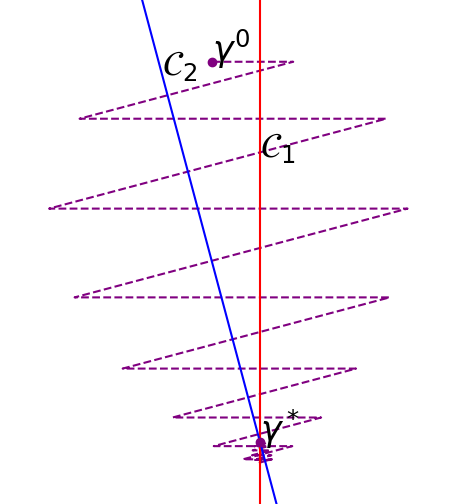
\includegraphics[width=5cm]{schema_c}
	\end{center}
	\caption{A wrapped figure going nicely inside the text.}\label{wrap-fig:1}
	\end{minipage}
	\begin{minipage}{0.49\textwidth}
		Optimal Transport is an efficient and flexible tool to compare two probability distributions. It has been popularized in the computer vision community in the context of discrete histograms \cite{Rubner2000}. The introduction of entropic regularization in \cite{cuturi13} has made possible the use of the fast Sinkhorn--Knopp algorithm \cite{sinkhorn64} scaling with high dimensional data.
	\end{minipage}
}


%----------------------------------------------------------------------------------------
%	Notations and definitions
%----------------------------------------------------------------------------------------

\headerbox{Sinkhorn-Knopp Algorithm}{name=Sinkhorn,column=0,below=intro}{
	We aim at numerically solving the entropic regularization of optimal transport~:
	\begin{equation} \label{eq:problem}
	\gamma^* = \argmin_{\gamma \in \Ccal_1 \cap \Ccal_2}
	\scal{c}{\gamma} + \epsilon \KL(\gamma,\One)
	\end{equation}
}


%----------------------------------------------------------------------------------------
%	
%----------------------------------------------------------------------------------------

\headerbox{Overrelaxation}{name=overrelaxation,column=1}{

}

%----------------------------------------------------------------------------------------
% Main result
%----------------------------------------------------------------------------------------

\headerbox{Lyapunov Function}{name=lyapunov,below=Sinkhorn,column=0}{
    
}


%----------------------------------------------------------------------------------------
%	Bootstrap
%----------------------------------------------------------------------------------------

\headerbox{Experiments}{name=expe,below=overrelaxation,column=1}{



}

%----------------------------------------------------------------------------------------
%	REFERENCES
%----------------------------------------------------------------------------------------


\headerbox{References}{name=references,below=lyapunov,span =2}{
\noindent [1] M. Cuturi. Sinkhorn distances: Lightspeed computation of optimal transport. {\it Advances in Neural Information Processing Systems 26}, 2013.\\
...
}



\end{poster}

\end{document}